 
\section*{Aufgabe 1: \emph{Maxwell'sche Geschwindigkeitsverteilung}}


\section*{Aufgabe 2: \emph{Zufallszahlengeneratoren}}

Zufallszahlengenerator mit
\begin{equation}
x_n=(ax_{n-1}+b) \text{mod}m.
\end{equation}

\begin{itemize}


\item[a)] $a=1601$, $b=3456$, $m=10000$.
\item[b)] Das Ergebnis hängt nur vom Startwert ab, wenn dieser nicht in dem vorherigen Array (was ist damit gemeint?) enthalten ist.
\begin{figure}
\centering
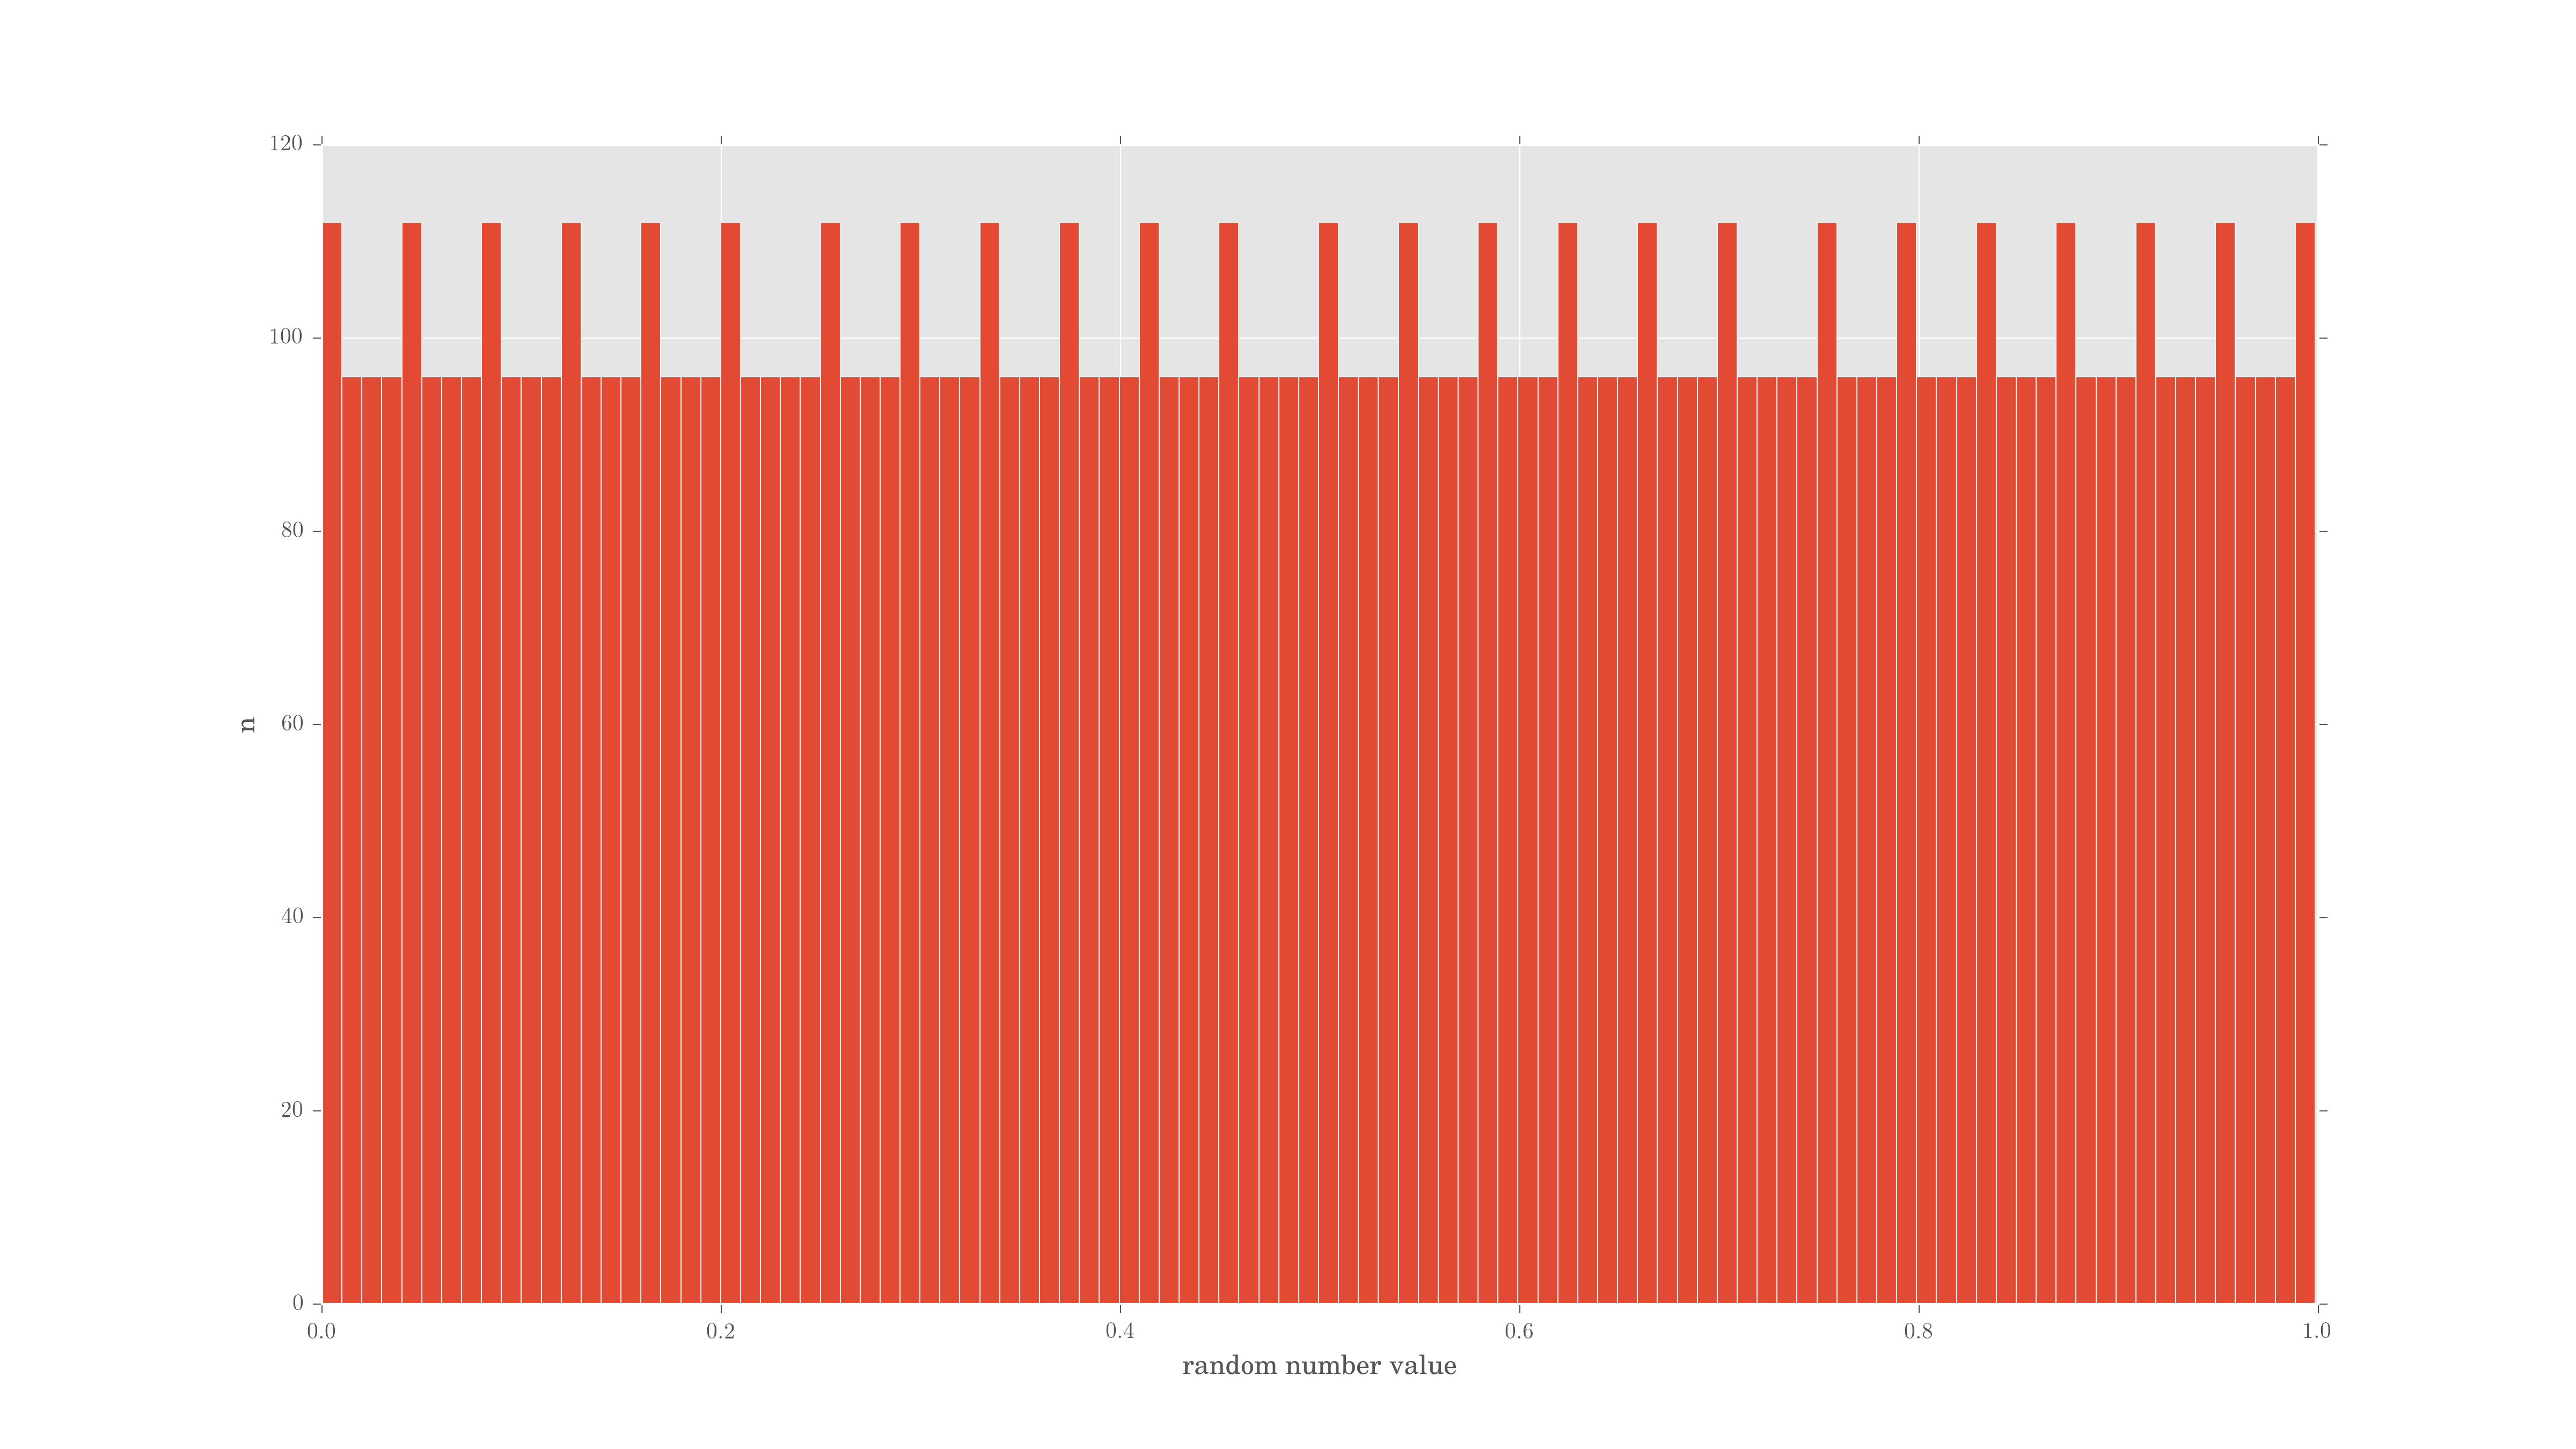
\includegraphics[width=\textwidth]{linear_kongruent_random_numbers.png}
\caption{$10000$ Zufallszahlen, erzeugt mit dem in Aufgabenteil a) programmierten Zufallszahlengenerator.}
\label{fig:2b}
\end{figure}
\item[c)] In den Histogrammen sind eindeutig Strukturen (Linien oder Ebenen) zu erkennen. Dies deutet darauf hin, dass Zahlen von den vorher generierten Zahlen abhängen und nicht komplett gleichverteilt sind.
\begin{figure}
\centering
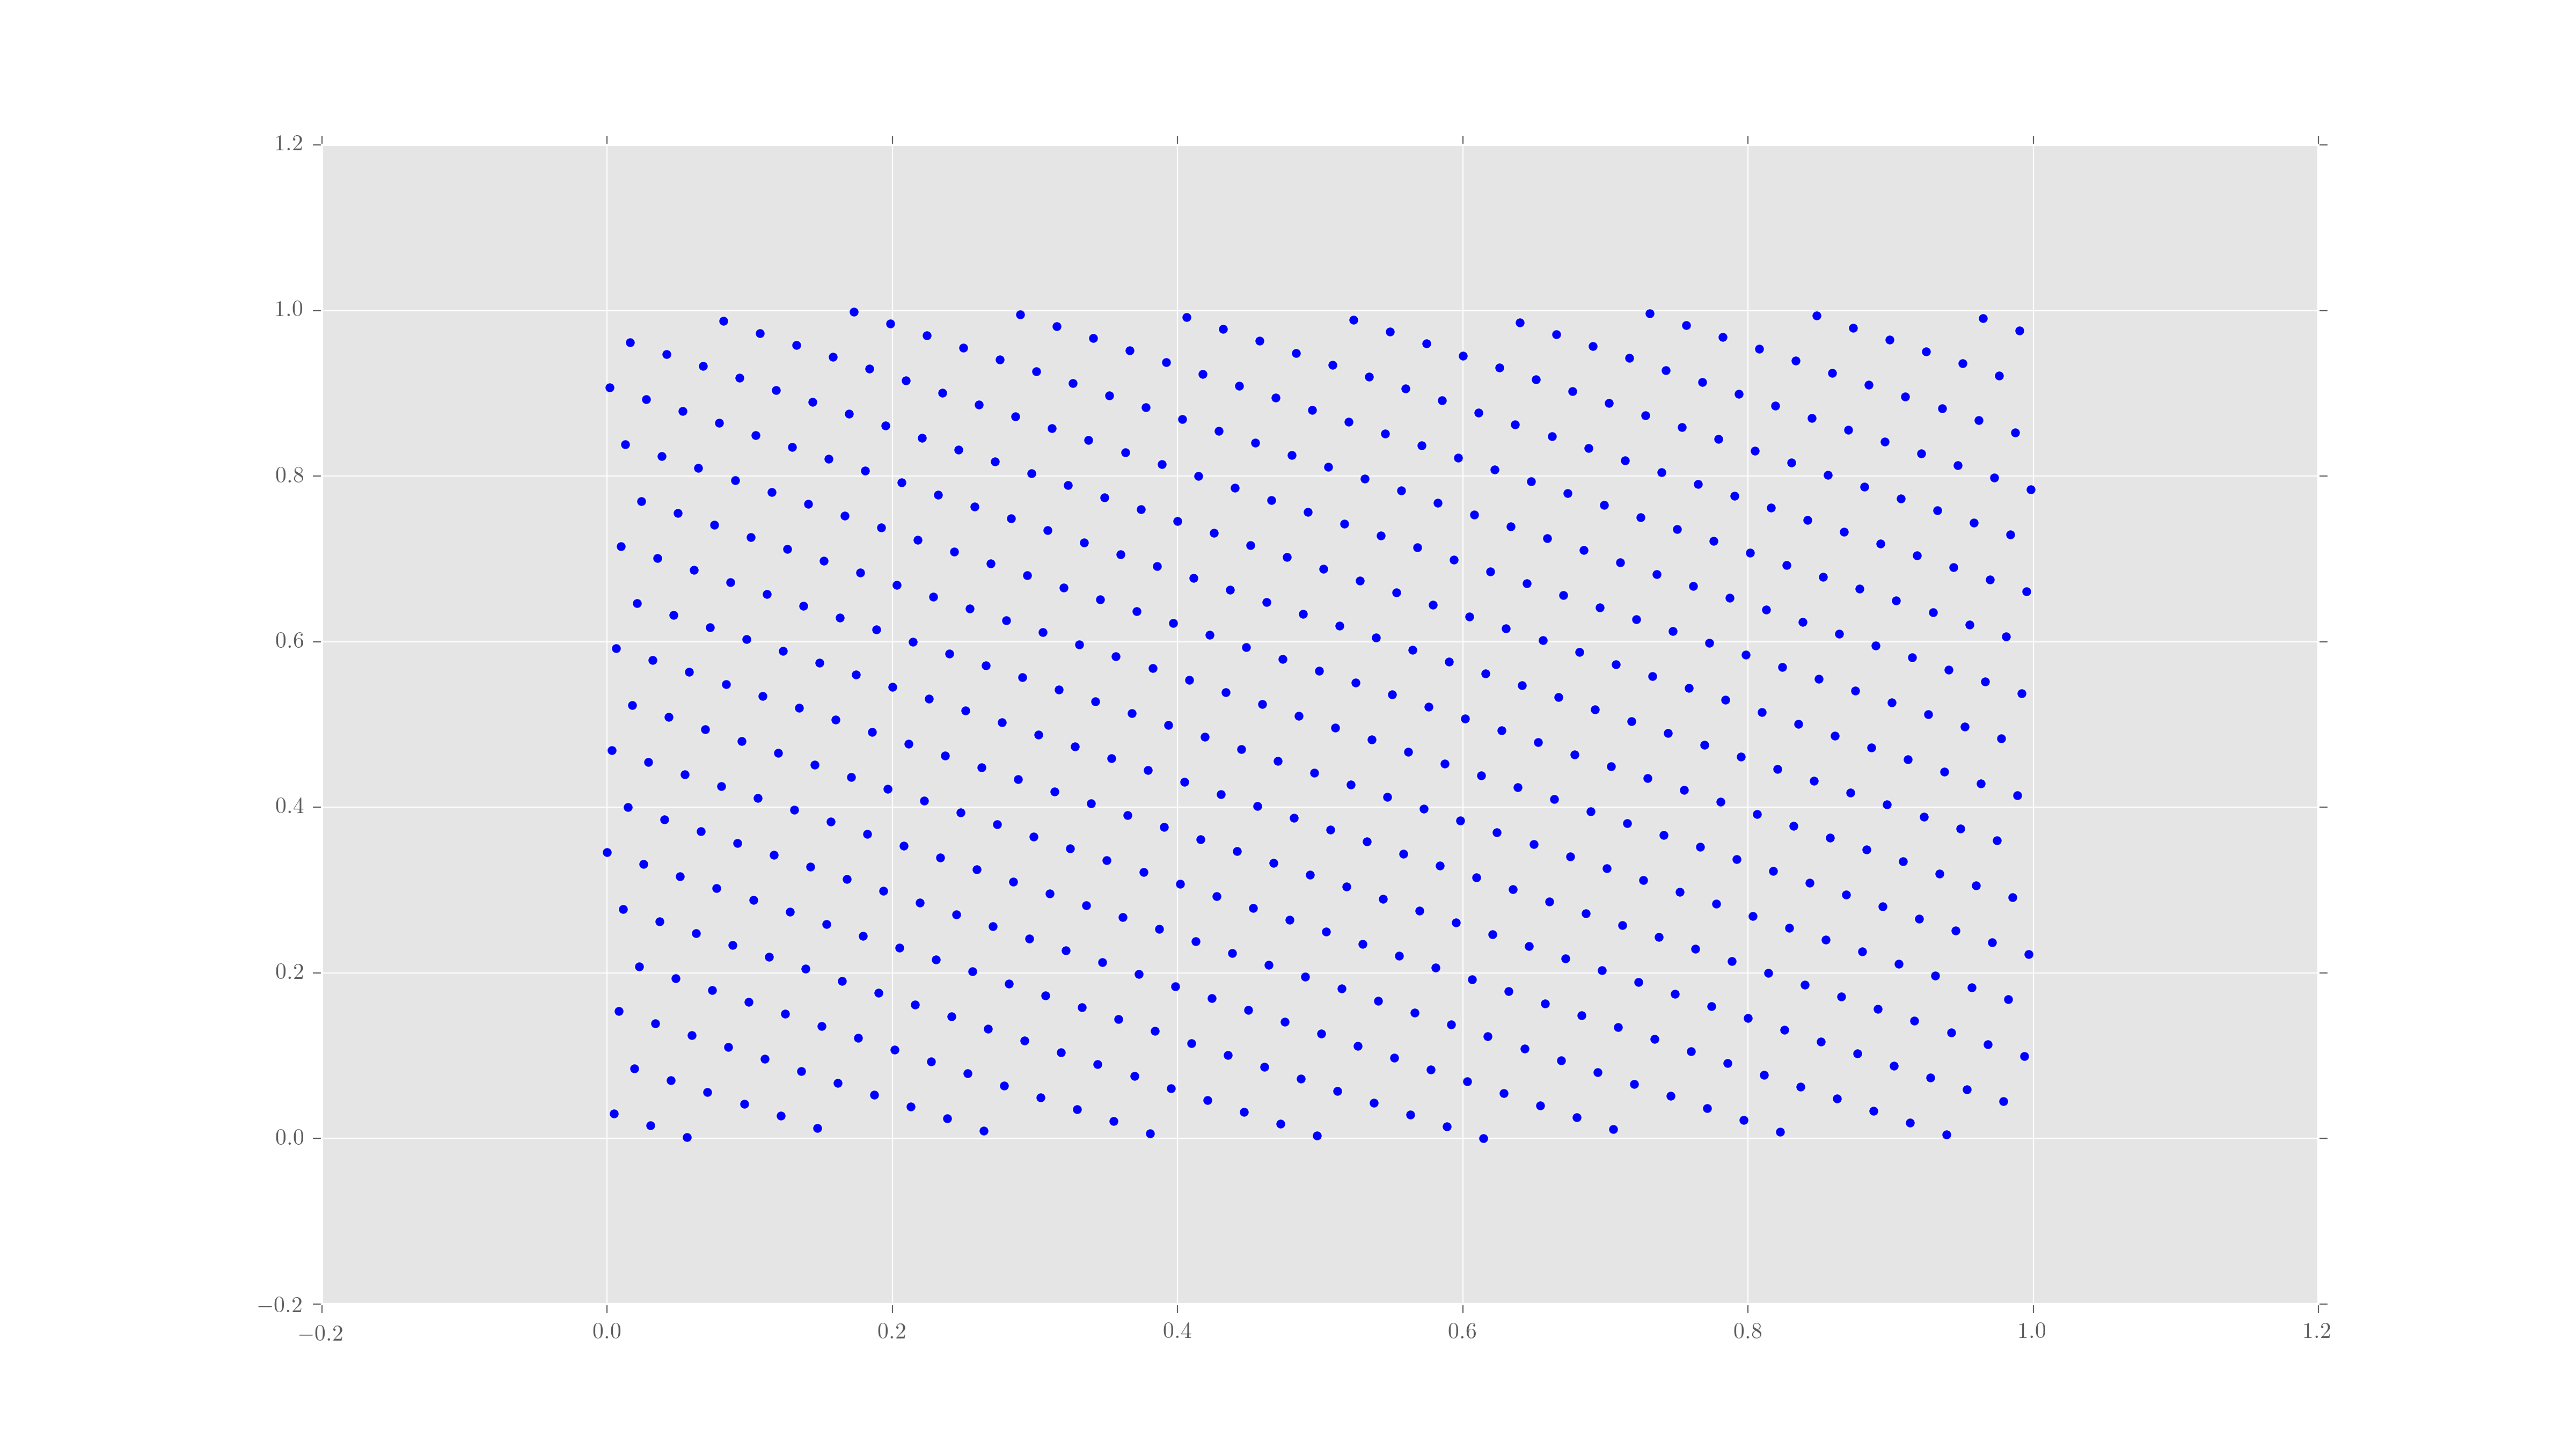
\includegraphics[width=\textwidth]{2dscatter.png}
\caption{Paare von Zufallszahlen, dargestellt als zweidimensionales Histogramm.}
\label{fig:2c1}
\end{figure}

\begin{figure}
\centering
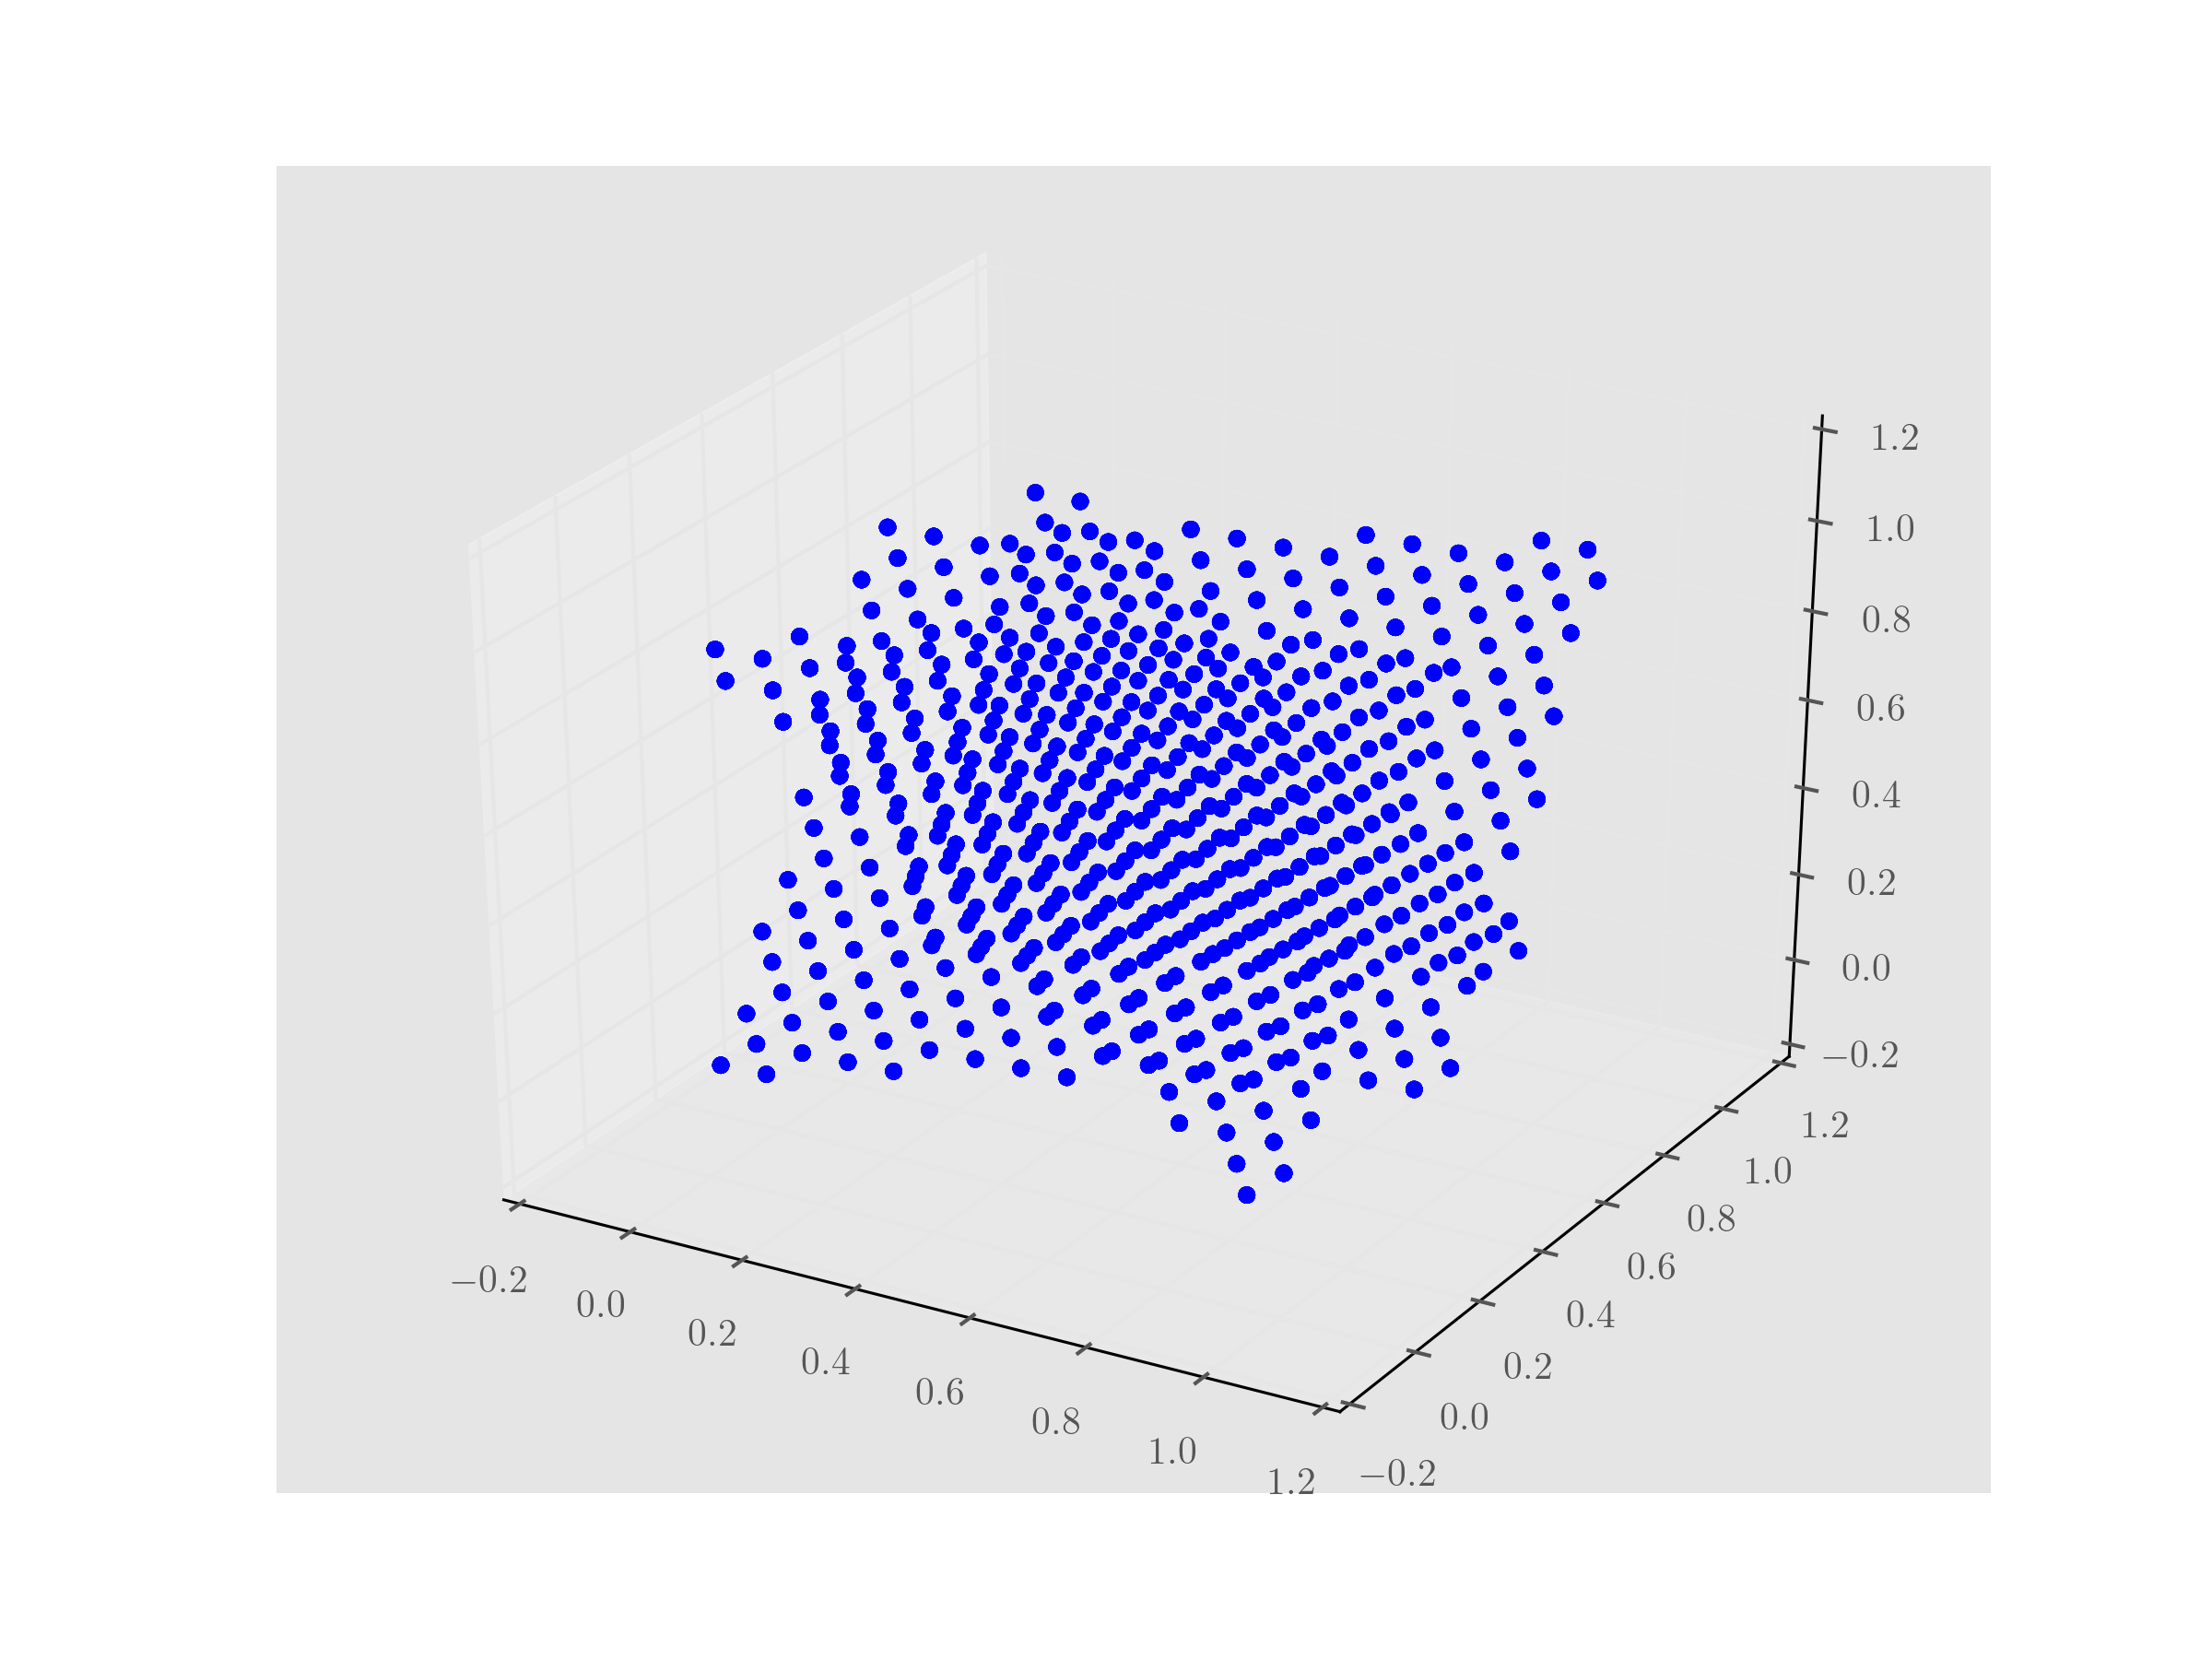
\includegraphics[width=\textwidth]{3dscatter.png}
\caption{Tripel von Zufallszahlen, dargestellt als zweidimensionales Histogramm.}
\label{fig:2c2}
\end{figure}
\item[d)]

\item[e)] 

\begin{figure}
\centering
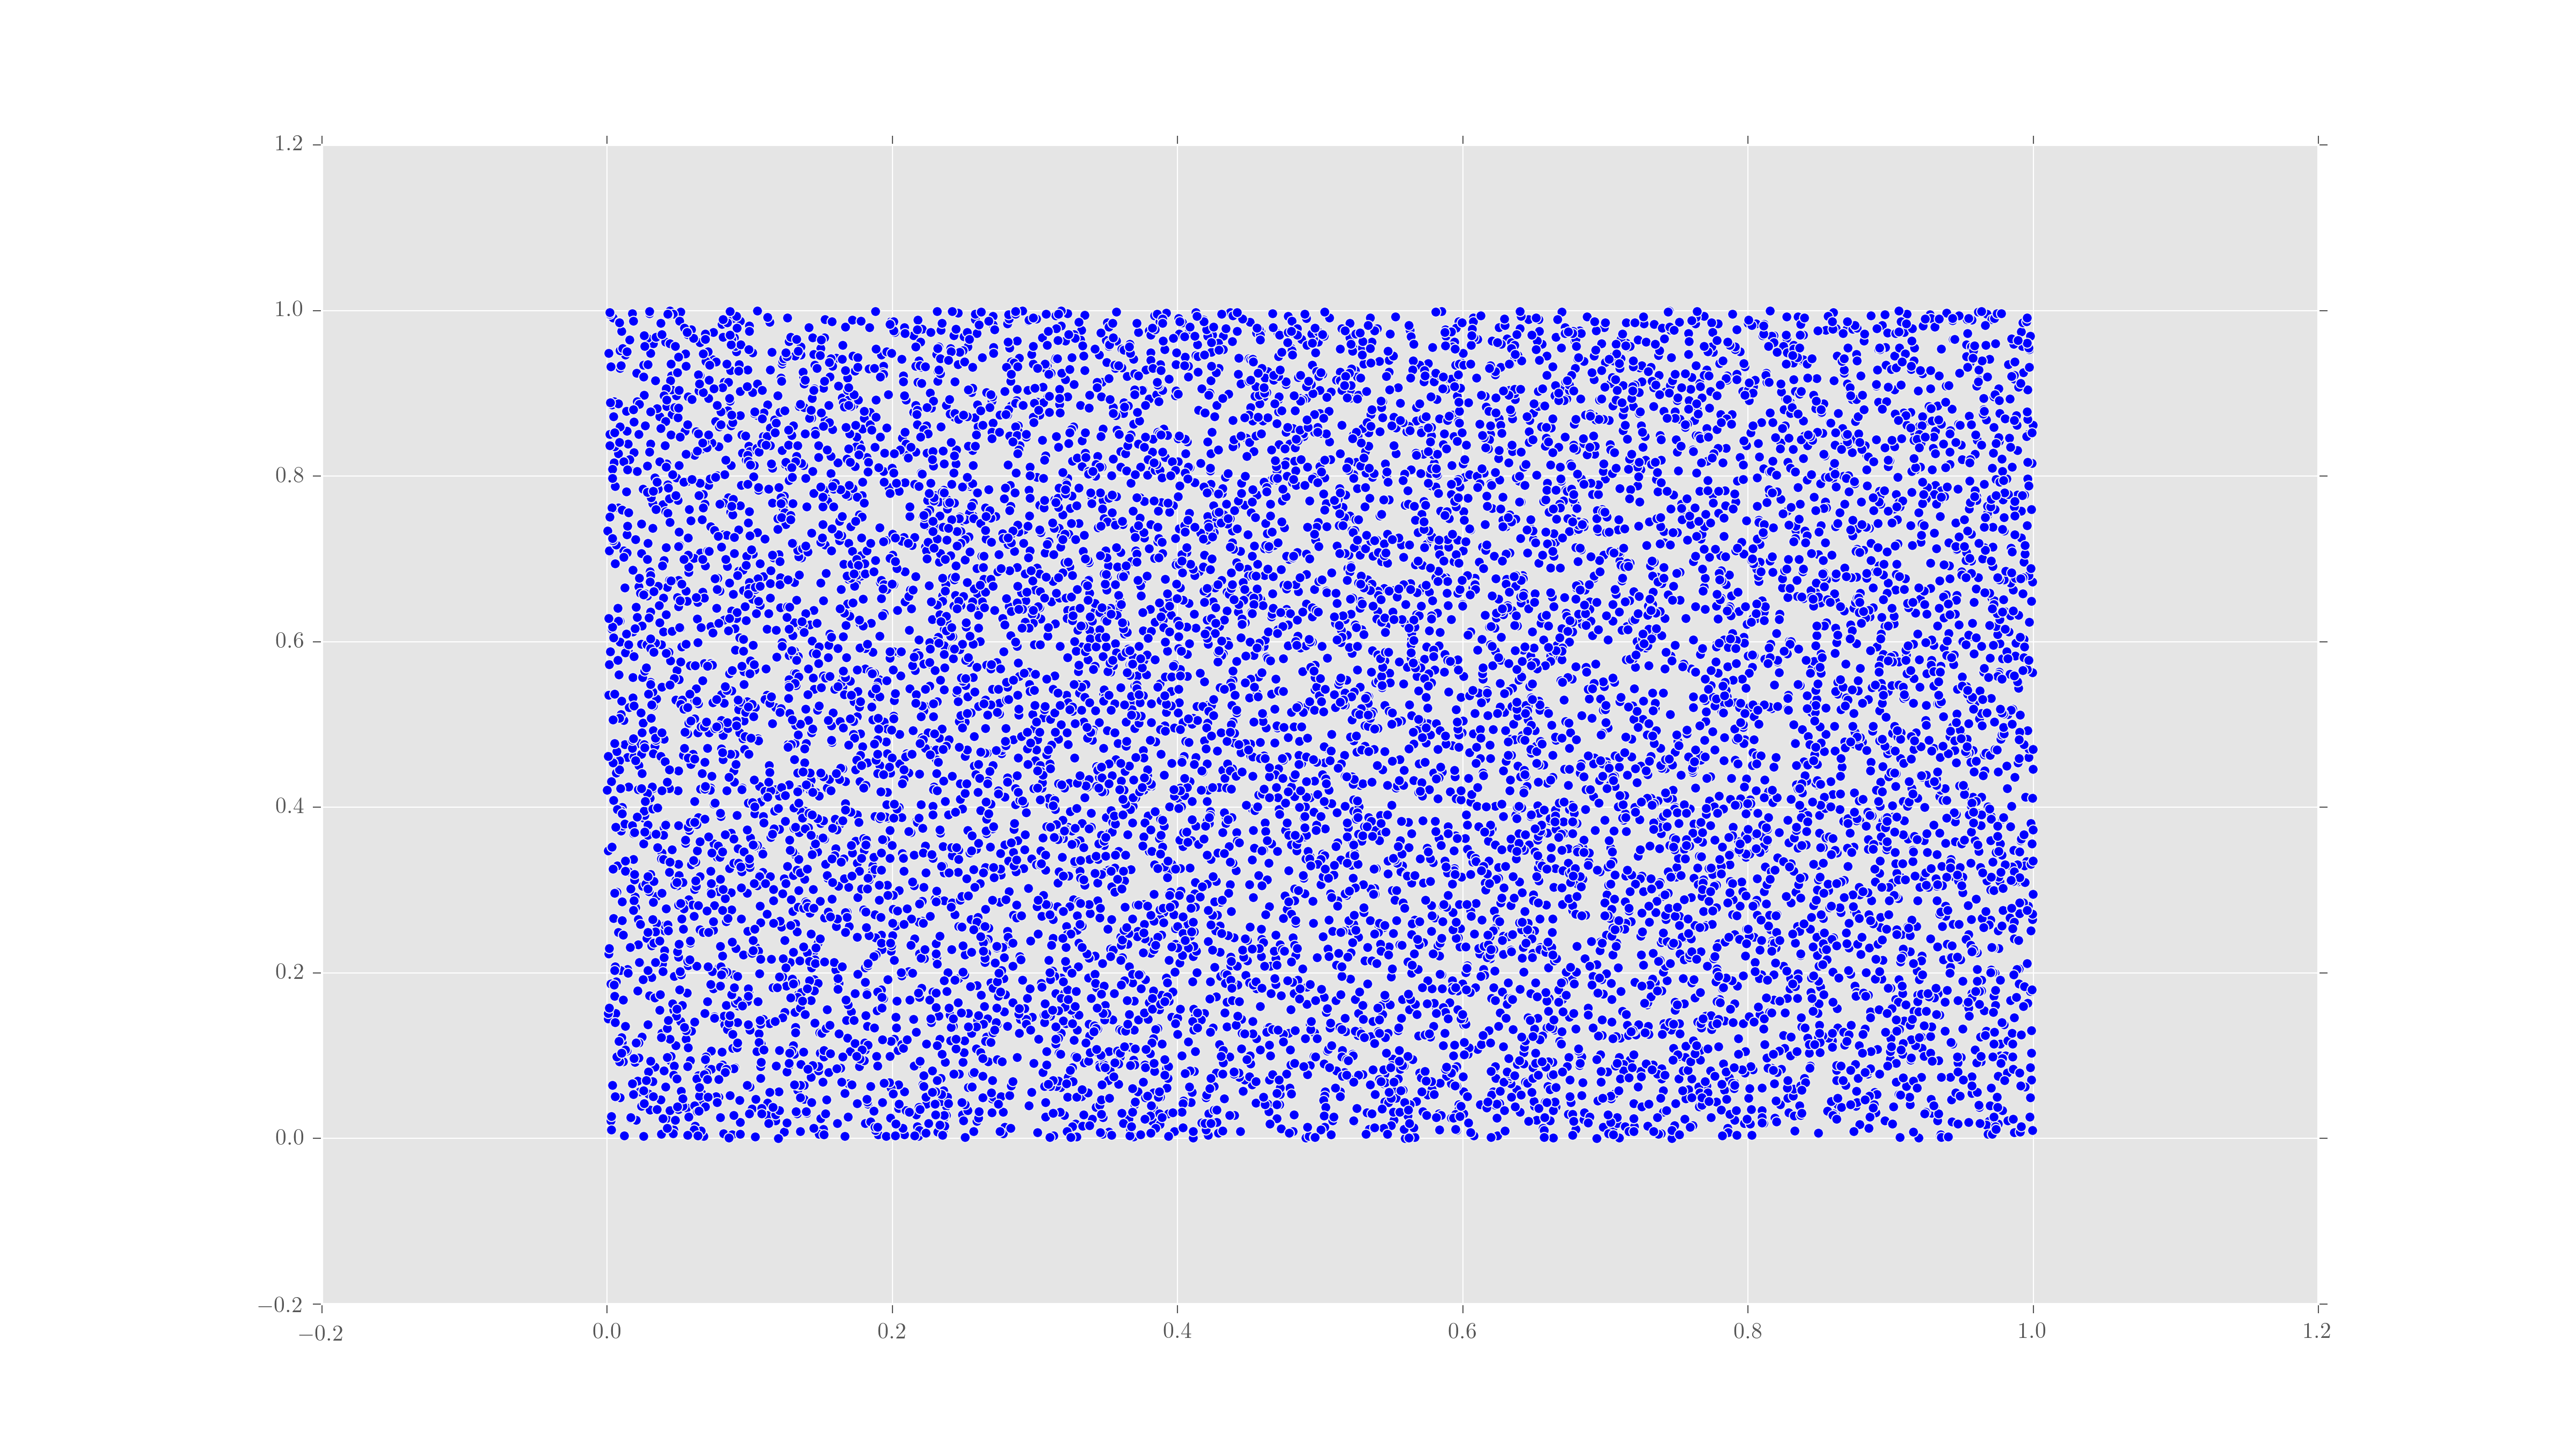
\includegraphics[width=\textwidth]{2dscatter_root.png}
\caption{Tripel von Zufallszahlen, dargestellt als zweidimensionales Histogramm. Im Gegensatz zu dem vorherigen zweidimensionalen Histogramm lässt sich hier keine Struktur erkennen.}
\label{fig:2e1}
\end{figure}

\begin{figure}
\centering
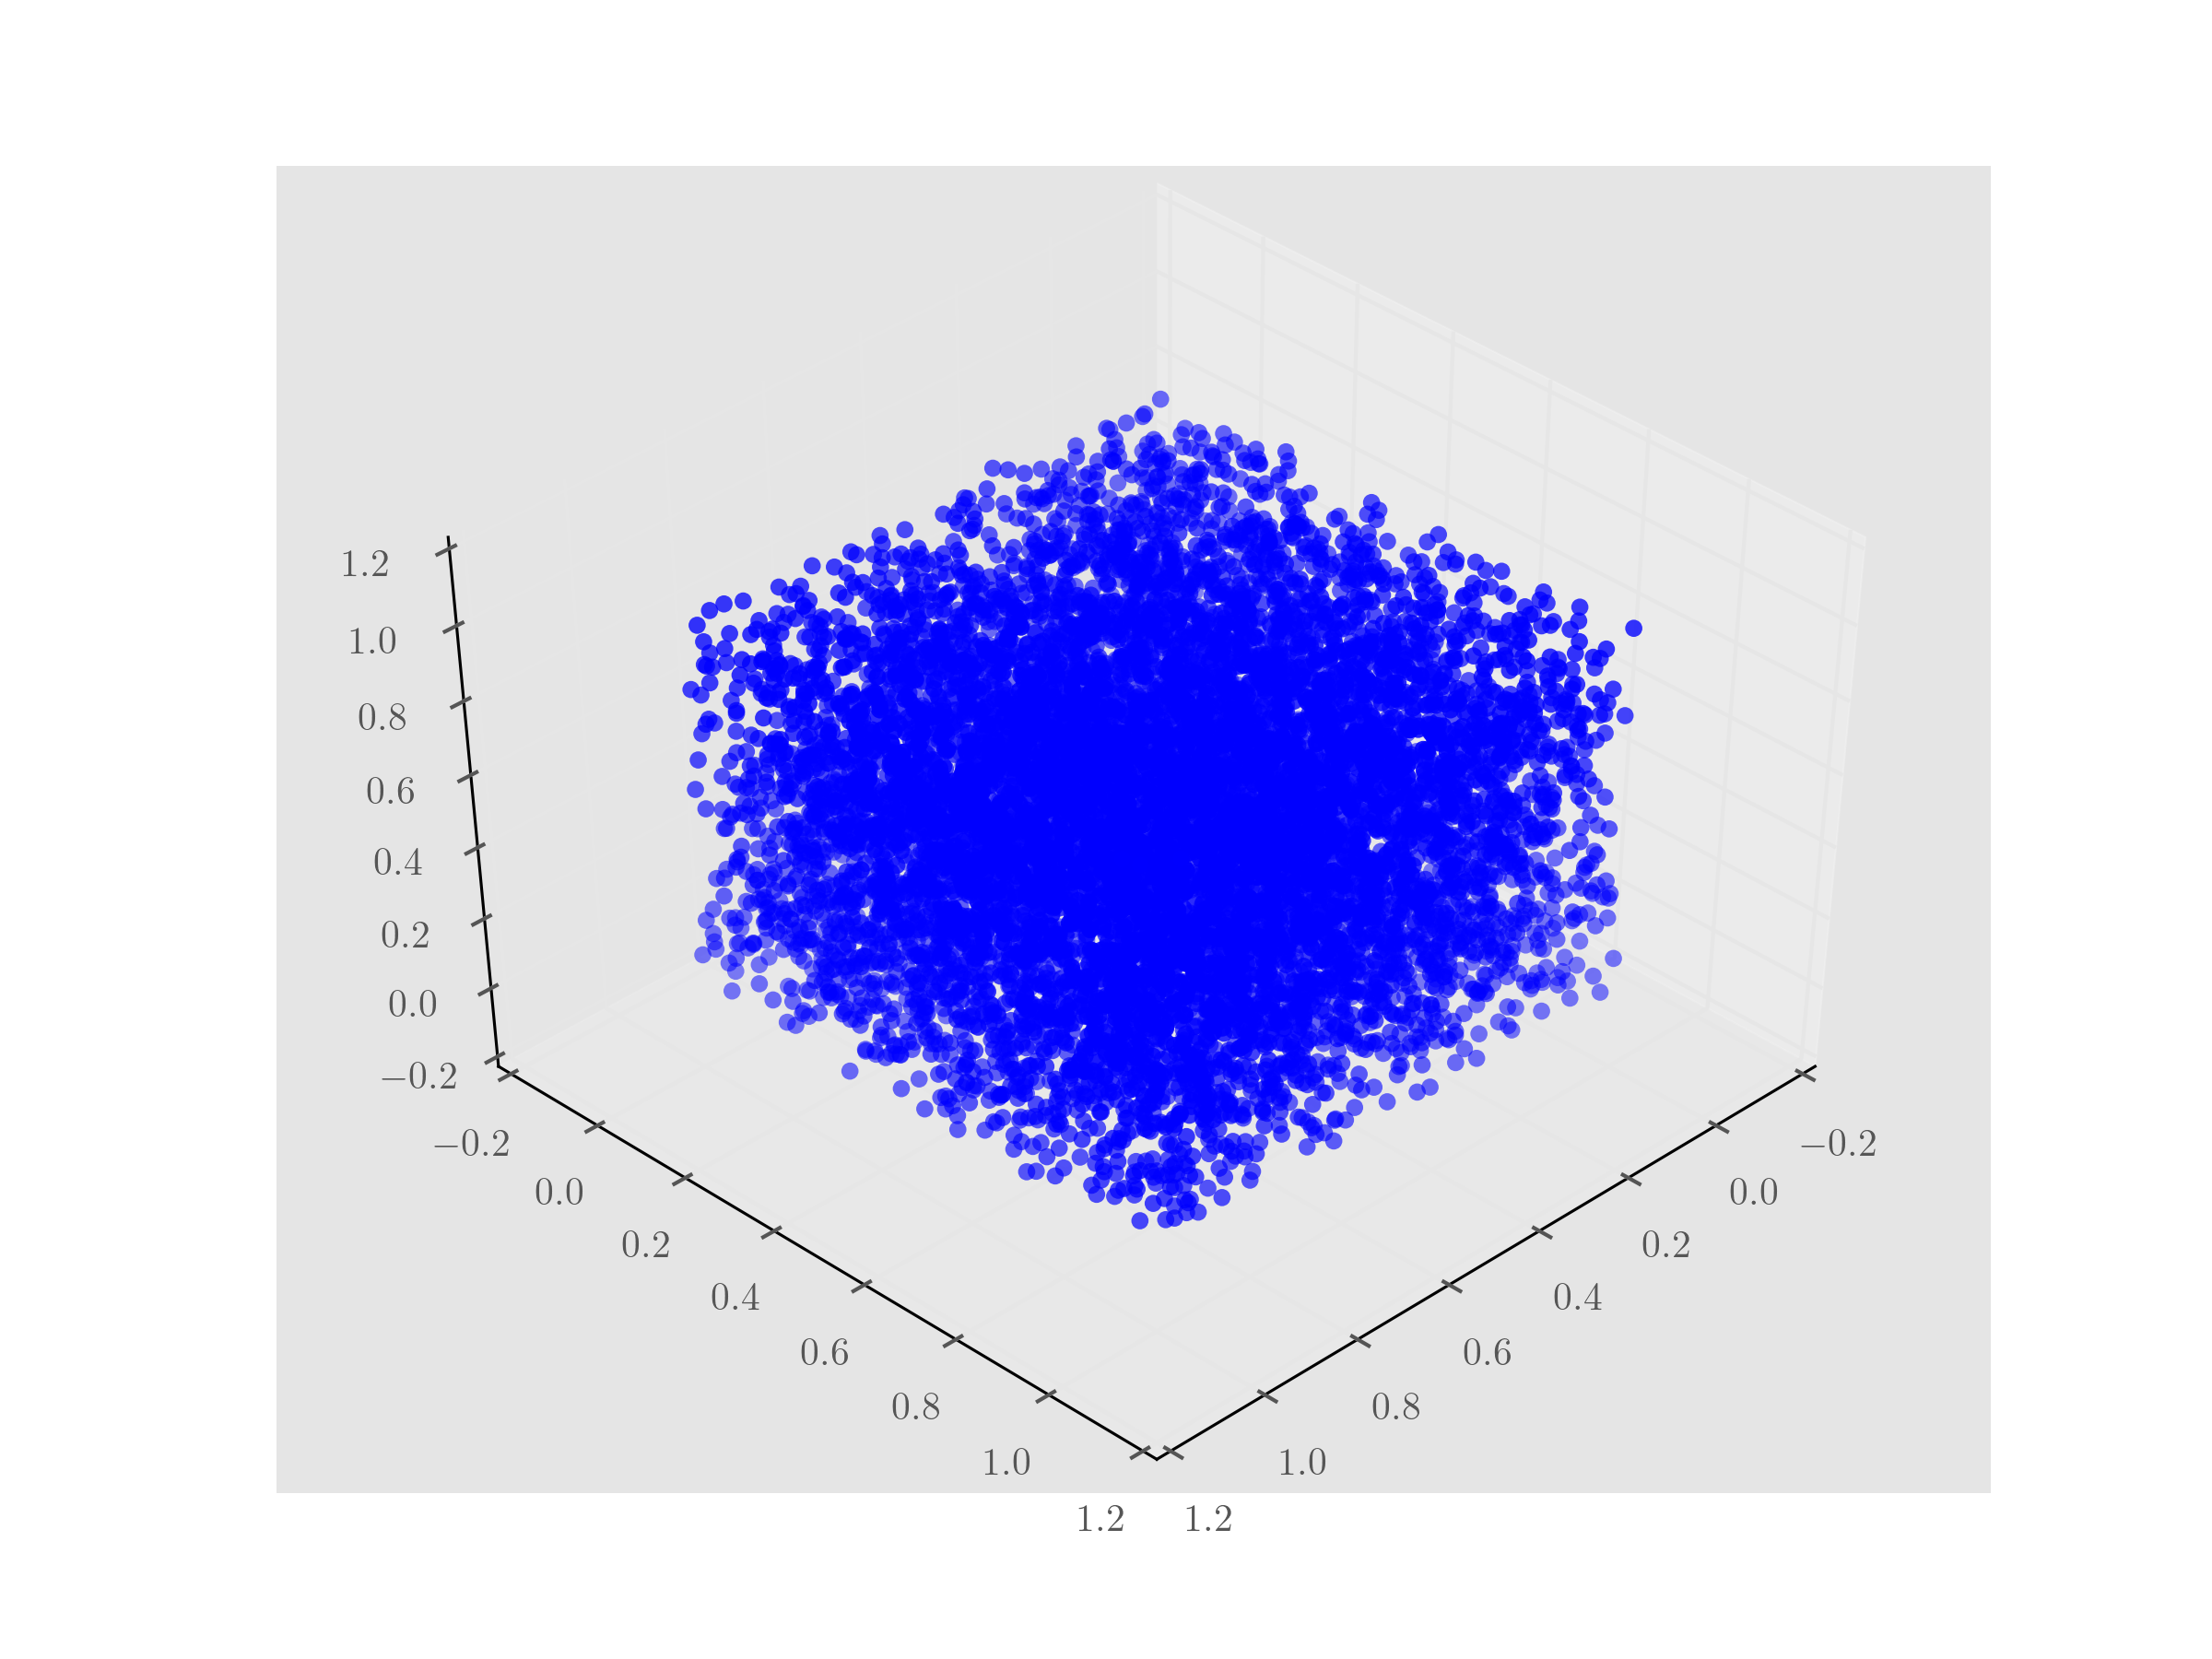
\includegraphics[width=\textwidth]{3dscatter_root.png}
\caption{Tripel von Zufallszahlen, dargestellt als dreidimensionales Histgramm.Im Gegensatz zu dem vorherigen dreidimensionalen Histogramm lassen sich hier keine Ebenen erkennen.}
\label{fig:2e2}
\end{figure}
\item[f)] Nur, wenn seed/m = 0.5.

\end{itemize}

\section*{Aufgabe 3: \emph{Zufallszahlengeneratoren}}


\section*{Aufgabe 4: \emph{Fehlerfortpflanzung}}
\begin{itemize}

\item[a)]

\begin{align}
y=a_0+a_1x\\
a_0=a_1=1.0\pm0.2\\
\rho = \frac{\text{cov}(a_0,a_1)}{\sigma(a_0)\sigma(a_1)}=-0.8\\
\text{cov}(a_0,a_1)=\rho \sigma(a_0)\sigma(a_1)=-0.8\cdot 0.2\cdot 0.2 = 0.032\\
\sigma_{y_1}=\sqrt{\left(\frac{\partial y}{\partial x}\sigma_x\right)²} = \sqrt{{a_1}²{\sigma_x}²}=0.2\\
\sigma_{y_2}=\sqrt{\left(\frac{\partial y}{\partial x}\sigma_x\right)²+2\frac{\partial y}{\partial x}\text{cov}(a_0,a_1)}=\sqrt{{a_1}²{sigma_x}²+2a_1\text{cov}(a_0,a_1)}=\sqrt{0.2²+1\cdot 0.032}=0.3224
\end{align}
\end{itemize}